\documentclass[10pt,letterpaper]{article}
\usepackage[left=1.8cm, right=1.8cm, top=1cm]{geometry}
\usepackage[utf8]{inputenc}
\usepackage[T1]{fontenc}
\usepackage[spanish]{babel}
\usepackage{amsmath}
\usepackage{amsfonts}
\usepackage{amssymb}
\usepackage{graphicx}
\usepackage{subfigure}
\usepackage{steinmetz}
\usepackage{float}
%\usepackage{circuitikz}

\author{Clase Práctica $\#$6}
\title{Electrónica I}
\date{Serie y transformada de Fourier. Sistemas lineales e invariantes en el tiempo. Filtros pasivos.}

\renewcommand{\sin}{\sen}
\begin{document}
	\maketitle
	
Bibliografía: Análisis de circuitos en ingeniería. Hayt \textit{et al.} 8va ed. Capítulos 16 y 18.

Probability, Random Variables and Random Signals Principles. Peyton Z. Peebles. 4ta ed. Capítulo 8.
\\

1- Muestre que para un sistema lineal e invariante en el tiempo (LTI) con respuesta al impulso $h(t)$, una entrada $x(t)$ puede relacionarse con su salida $y(t)$ mediante $y(t)=h(t)\ast x(t)$.

b) Si $\mathrm{Y}(\omega)=\mathcal{F}\{y(t)\}$, muestre que $\mathrm{Y}(\omega) = \mathrm{H}(\omega)\mathrm{X}(\omega)$.

c) Obtenga la función transferencial de un sistema formado por dos sistemas LTI en cascada cuyas respuestas al impulso son conocidas. \\

2- Sea una tensión periódica $v_s(t) = 40 \mathrm{V}$ para $0 < t < \dfrac{1}{96}$, y 0 para $\dfrac{1}{96} < t < \dfrac{1}{16}$ calcule:

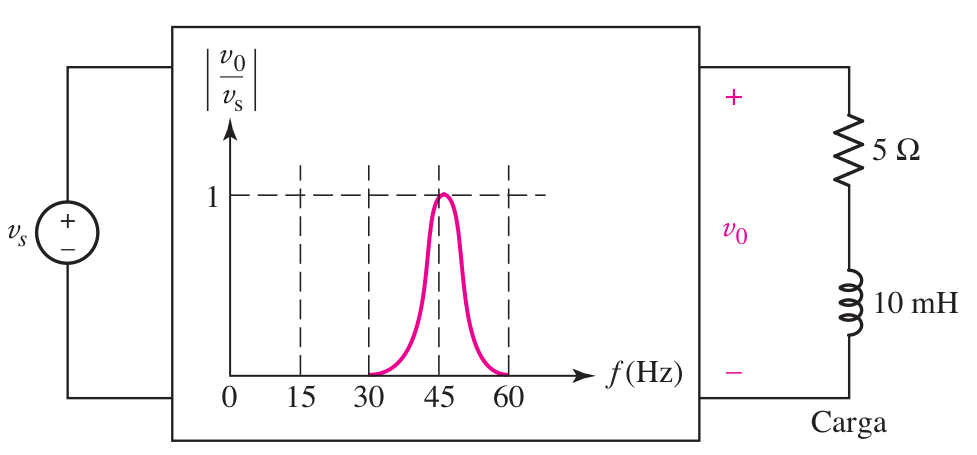
\includegraphics[scale=0.3]{c2.png}

a) El coeficiente de la serie de Fourier para $f=3f_0$, \textbf{$c_3$}.

b) La potencia entregada a la carga en el circuito de la figura. \\

3- Diseñe un filtro RC pasa alto con frecuencia de corte en 3 kHz. \\

4- Diseñe un filtro de pasa banda con un ancho de banda de 1 MHz y una frecuencia de corte nivel alto de 1,1 MHz.\\

5- De acuerdo con la figura, halle la la función transferencial $H(s)=\mathrm{V}_C/\mathrm{I}_s$ y grafique la respuesta en frecuencia (puede auxiliarse de un asistente matemático).

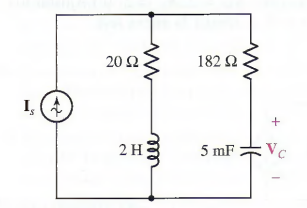
\includegraphics[scale=0.6]{c5.png}

 
\end{document}